\subsubsection{Harvester-Tarpit}
Das Skript \emph{reply.php}generiert, wie uter Punkt \ref{subsub:harverster-tarpit} beschrieben, neben neuen Hyperlinks auch durchschnittlich fünf bis zehn E-Mail-Adressen, welche von einem potentiellen Harvester eingesammelt werden können. Hierbei wurden innerhalb dieses achtmonatigen Betriebes über 300 E-Mails empfangen.\\
Vor allem eine E-Mail, besser gesagt eine regelrechte Spamwelle fiel hier besonders auf. Am 16. März 2018 kamen innerhalb von zwei Stunden rund 225 E-Mails an; sechs Tage später, am 22. März, folgten weitere 68 Nachrichten. Diese 293 E-Mails hatten alle den selben Aufbau: Adressiert an verschiedene Adressen, welche allesamt vom PHP-Skript generiert wurden, stammten sie von der \emph{Wolseley Industrial Group} und forderten den Empfänger auf eine Rechnung (Purchasing Order, PO) nochmals zu überarbeiten, zu bezahlen und an eine gewisse Helen Costanzo zurückzuschicken. Der E-Mail sind auch noch zwei Dokumente beigefügt.
\begin{figure}[H]
	\centering
	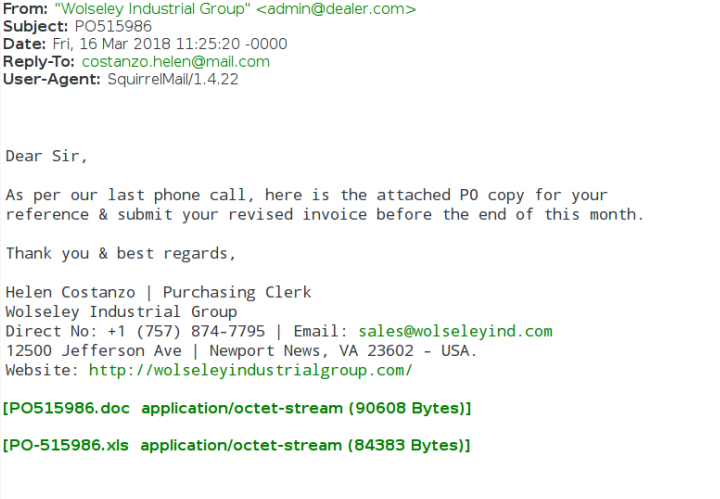
\includegraphics[width=8.45cm]{img/wolseley-industrial-group.png}
	\caption{E-Mail von der Wolseley Industrial Group}
	\label{fig:Wolseley_Industrial_Group}
\end{figure}
Die E-Mail, ersichtlich in Abbildung \ref{fig:Wolseley_Industrial_Group}, erscheint auf den ersten Moment glaubwürdig, denn die Wolseley Industrial Group ist ein in Amerika angesiedeltes Unternehmen und Helen Costanzo ist ein glaubwürdiger Name, vor allem für eine Angestellte eines amerikanischen Unternehmens. Vor allem die Signatur der E-Mail wirkt durch die echten Daten des Unternehmens authentisch. Die Signatur einer E-Mail kann man jedoch heutzutage mit nahezu jedem E-Mail-Programm einfach bearbeiten und somit fälschen. Bei genauerem Hinsehen erkennt man jedoch schnell, dass diese E-Mail gefälscht ist. Als Absender versteckt sich hinter den Namen Wolseley Industrial Group die E-Mail-Adresse \emph{admin@dealer.com}. Diese E-Mail-Adresse taucht auch als Absender anderer dubioser E-Mails auf, unter anderem auch bei einem \glqq Offiziellen Gewinnerbrief\grqq\space einer Lotterie.\cite{gewinnerbrief-admin-dealer} Am 22. März 2018 warnte auch die Wolseley Industrial Group selbst vor gefälschten E-Mails in ihrem Namen.\cite{scam-warnung-wolseley} Das Unternehmen warnt hierbei ausdrücklich davor, die angefügten Dateien zu öffnen, da sie mit Viren belastet sein könnten. Das Unternehmen bezeichnet diese Nachricht hierbei als eine Scam-Mail, also eine E-Mail, in welcher aufgefordert wird einen gewissen Geldbetrag zu bezahlen, um dann zu einem späteren Zeitpunkt daraus irgendeinen materiellen oder finanziellen Gewinn zu erzielen. Der deutsche Fachausdruck hierfür ist \emph{Vorschussbetrug} und ist strafbar.\cite{vorschussbetrug}\\
Welcher Harvester für das Sammeln der E-Mail-Adressen, an welche diese Scamnachrichten geschickt wurden, verantwortlich ist, lässt sich nicht mehr zurückverfolgen. Da zu diesem Zeitpunkt der E-Mail-Adressen-Präfix mit dem Unix-Timestamp, wie unter Punkt \ref{subsub:harverster-tarpit} erwähnt, noch nicht implementiert wurde und ein Harvester diese Adressen zu jedem beliebigen Zeitpunkt X oder gar über mehrere Wochen verteilt gesammelt haben könnte, kann man im Nachhinein nicht mehr zweifelsfrei feststellen, welcher Harvester die betroffenen Adressen eingesammelt hat. Auch das betroffene Unternehmen gibt hierzu keine näheren Auskünfte.
%TODO: EVTL. EINBAUEN
%Ein IP-Lookup\footnote{Bei einem IP-Lookup wird die IP-Adresse zurückverfolgt und man erhält somit Informationen über Besitzer, ungefähren Standort des Endgerätes und vieles mehr.} hat jedoch ergeben, dass die E-Mails von einem Mailserver aus gesendet wurden, welcher in Dallas, Texas steht.
\\Bereits wenige Wochen später, am 12. April 2018, wiederholte sich der zuvor genannte Vorfall: Eine E-Mail, diesmal vom Unternehmen \emph{Bearing Distributors Inc}, fordert den Empfänger auf, die mitgeschickte Rechnung zu überprüfen und an eine Costanzo Helen zurückzuschicken. Das betroffene Unternehmen hat sich bislang (14. April 2018) noch nicht zum Vorfall geäußert.
%TODO: SOGEN DASS LEI E-MAIL ADRESSEN MIT S,A,N,O UNGRBM WORDN SAN UND A POOR NO MIT R UND P
%TODO: DE MARXISMUS-MAIL ERWÄHNEN